\documentclass[tikz,border=2mm]{standalone}
\usepackage{tikz}
\usepackage{pgfplots}
\pgfplotsset{compat=1.18}

% Definir estilo para el gráfico
\pgfplotsset{
    mybar/.style={
        ylabel=,  
        xlabel=,
        x tick label style={font=\tiny},
        yticklabel style={font=\tiny},
        ymin=0,
        enlarge x limits=0.12,
        ybar=4pt,
        bar width=5pt,
        symbolic x coords={Código, Confluence, S. ficheros, G. Drive, GitLab},
        xtick={Código, Confluence, S. ficheros, G. Drive, GitLab},
        x tick label style={rotate=45, anchor=east, font=\scriptsize},
        width=6cm,
        height=5cm,
        grid=major,
        grid style={dashed, gray!30},
        tick label style={font=\scriptsize},
        legend style={draw=none},
        scale only axis,
        title={LLM juez},
        title style={font=\normalsize}
    }
}

\begin{document}
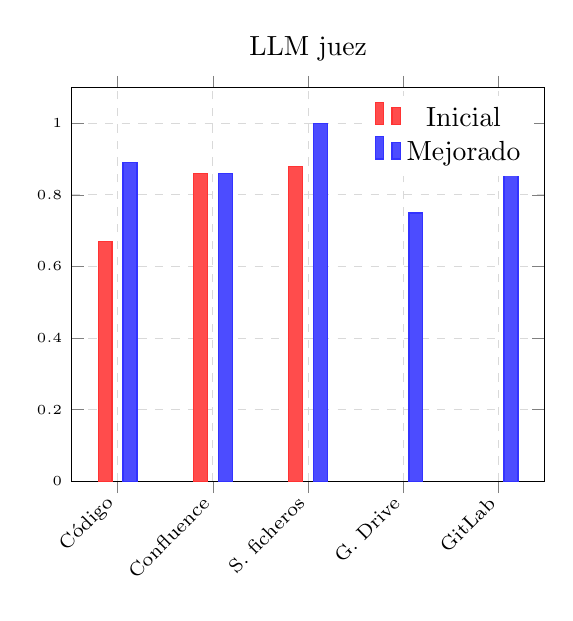
\begin{tikzpicture}
\begin{axis}[
    mybar,
    ymax=1.1,
    ytick={0,0.2,0.4,0.6,0.8,1.0},
]
\addplot[
    fill=red!70,
    draw=red!80,
    line width=0.5pt
] coordinates {
    (Código, 0.67)
    (Confluence, 0.86)
    (S. ficheros, 0.88)
};
\addplot[
    fill=blue!70,
    draw=blue!80,
    line width=0.5pt
] coordinates {
    (Código, 0.89)
    (Confluence, 0.86)
    (S. ficheros, 1.0)
    (G. Drive, 0.75)
    (GitLab, 0.9)
};
\legend{Inicial, Mejorado}
\end{axis}
\end{tikzpicture}
\end{document}
